\documentclass{standalone}
\usepackage{textcomp}
\usepackage{pgfplots}
\begin{document}
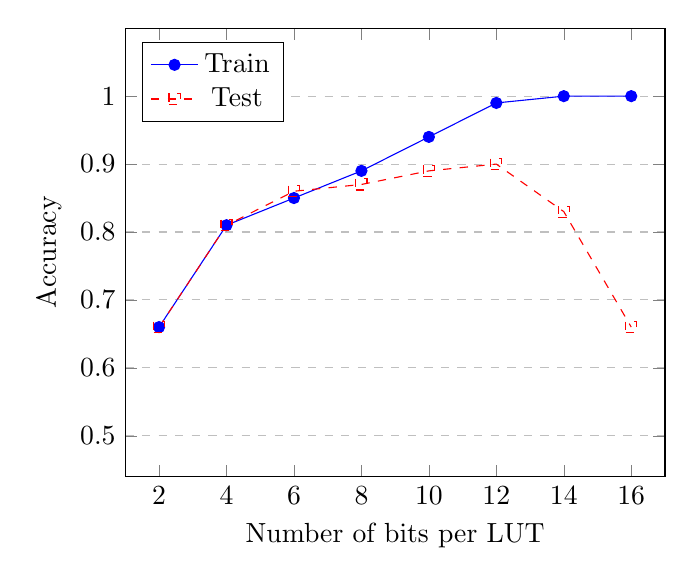
\begin{tikzpicture}
\begin{axis}[
    %title={Real data},
    xlabel={Number of bits per LUT},
    ylabel={Accuracy},
    xmin=1, xmax=17,
    ymin=0.44, ymax=1.1,
    xtick={2,4,6,8,10,12,14,16},
    ytick={0.5,0.6,0.7,0.8,0.9,1.00},
    legend pos=north west,
    ymajorgrids=true,
    grid style=dashed,
]

\addplot[
    color=blue,
    mark=*,
    ]
    coordinates {
        (2,0.66)(4,0.81)(6,0.85)(8,0.89)(10,0.94)(12,0.99)(14,1.00)(16,1.00)
    };
    \addlegendentry{Train}

\addplot[
    color=red,
    mark=square,
    dashed,
    ]
    coordinates {
        (2,0.66)(4,0.81)(6,0.86)(8,0.87)(10,0.89)(12,0.90)(14,0.83)(16,0.66)
    };
    \addlegendentry{Test}

\end{axis}
\end{tikzpicture}
\end{document}
